

%Here we use the beamer class instead of article. If we add in the optional [handout] line, all the \pause will be removed. This is useful if you want to create a version of your slides to be shared as a document. Otherwise every \pause creates a new page. Try it out to see the difference.
\documentclass{beamer}
%documentclass[handout]{beamer}


%This is an alternative way to add packages. More compact, but also more of a pain when you want to remove some.
\usepackage{tikz, tikz-cd}
\usepackage{amsmath,amssymb, amsthm, xcolor}
\usetikzlibrary{calc}
\usepackage{tcolorbox}
\usepackage{roboto}     %This is a font package I like


\def \FF {\mathbb{F}}
\def \ZZ {\mathbb{Z}}
\def \RR {\mathbb{R}}
\def \CC {\mathbb{C}}
\def \QQ {\mathbb{Q}}
\def \AA {\mathbb{A}}
\def \poly {\mathrm{Poly}}
\def \sfr {\mathrm{sf}}
\def\v{\vspace{.15in}}
\def \C {\mathcal{C}}
\def \PP {\mathbb{P}}
\def \NN {\mathbb{N}}
\def \PConf {\mathrm{PConf}}
\def \sgn {\mathrm{sgn}}
\def \E {\mathcal{E}}
\def \Std {\mathrm{Std}}
\def \ld {\lessdot}

\def \R {\mathcal{R}}
\def \M {\mathcal{M}}
\def \wt {\widetilde}
\def \U {\mathcal{U}}
\def \h {\widehat}
\def \H {\mathcal{H}}

\def \irr {\mathrm{Irr}}
\def\s{\hspace{.1em}}

\def\preper{\mathrm{PrePer}}

\newtheorem{thm}{Theorem}
\newtheorem{prop}[thm]{Proposition}
\newtheorem{conj}[thm]{Conjecture}
\newtheorem{defn}[thm]{Definition}
\newtheorem{cor}[thm]{Corollary}

\setbeamerfont{frametitle}{series=\bfseries}


%There are many themes you can choose from which dictate the style of the slides. I'm using default here.
\usetheme{default}

%We can define custom color names.
%The HTML tells LaTeX that we will be using a hex code to define our color. The {951829} is the hex for Vassar's official Burgundy.
\definecolor{VassarBurgundy}{HTML}{951829}
\definecolor{VassarDarkBurgundy}{HTML}{641A2B}
\definecolor{VassarCream}{HTML}{FFF8EF}

%These lines set the color defaults for structural parts of the slides. Try changing the colors to see what gets affected.
\setbeamercolor{frametitle}{bg=VassarBurgundy,fg=VassarCream}
\setbeamercolor{structure}{bg=VassarBurgundy,fg=VassarBurgundy}
\setbeamercolor{block title}{bg=VassarBurgundy,fg=VassarCream}

%Here are a few other colors I've used in the past, defined using RGB instead of hex.
\definecolor{forest}{RGB}{0,155,85}
\definecolor{techblue}{RGB}{46, 175, 255}
\definecolor{gold}{RGB}{218,165,32}
\definecolor{cyan}{RGB}{0,255,255}

%Let's create a new command for a large box with a Vassar color theme
\newcommand{\vassarbox}[1]{
    \begin{tcolorbox}[
     colback=VassarBurgundy,        % background color
     coltext=VassarCream,           % text text
     halign= center,                % horizontal alignment
     fontupper={\Huge \bfseries},   % Set the font here
     sharp corners,                 % no rounded corners for the box
     boxrule=0pt                    % turn off frame 
     ]{#1}
    \end{tcolorbox}
}


\begin{document}

%A beamer document consists of a sequence of frames (i.e. slides). I like to add some comments to help me visually deliniate where each new slide begins.

%%%%%%%%%%%%%%%%%%%%%%%%%%%%%%%%%%%%%%%%%%%%%%
% FRAME 

%In this title slide I've added in a semi-transparent background image.
{\usebackgroundtemplate{
    \tikz\node[opacity=0.3]{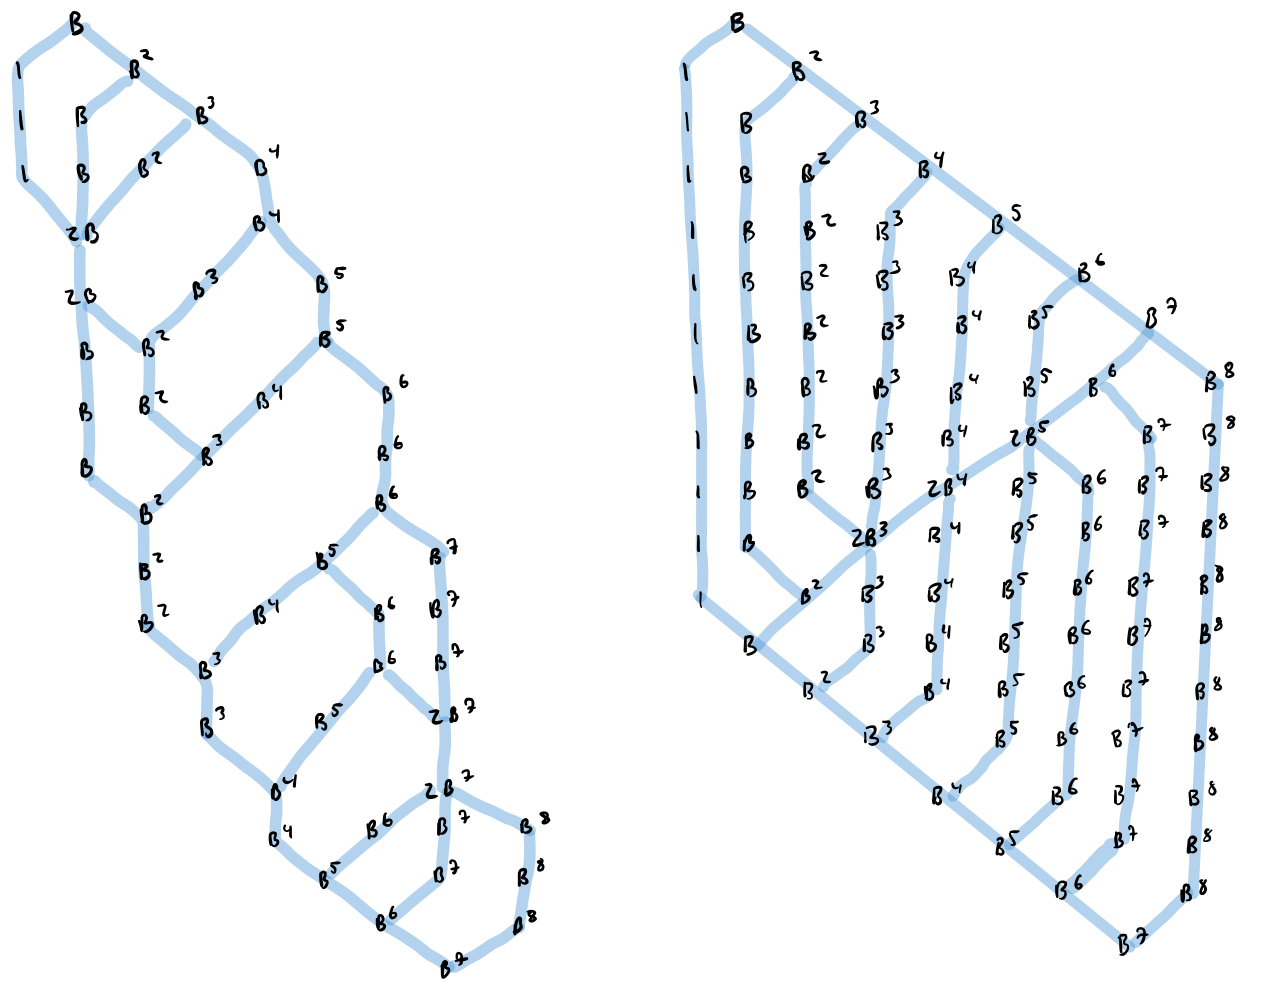
\includegraphics[width=\paperwidth]{figs/proofs.png}};}
    \begin{frame}
        \vassarbox{Let's Learn \LaTeX\\Level 4}
        
        \begin{center}
            {\Large \bfseries Trevor Hyde\\ URSI 2025}
            \vspace{.4in}
            
            {\large \bfseries In which we learn\\ the basics of Beamer}
        \end{center}
    \end{frame}
}%This grouping limits the scope of the background image. Without it, the background gets applied to all the slides.

%%%%%%%%%%%%%%%%%%%%%%%%%%%%%%%%%%%%%%%%%%%%%%
% FRAME 

\begin{frame}{What is Beamer?} %The text in this box gets added as the heading 
    Beamer is a ``document class'' in LaTeX which allows you to create slide decks. 
    Some of the benefits include:
    
    \begin{itemize}
        \pause %Adding a \pause will split the frame into multiple pages so you can click to reveal the text. A lot of people like this, but I caution against using too much.
        \item Scalability: slides look great at large resolutions, which is ideal when your slides will be on a big screen.
        You can be sure that your slides will look the same on this screen as they will on the big screen.
        \pause
        \item Math: we get all the power and control of making professional looking math but now in a slide deck.
        \pause
        \item Easy to edit: once you get past the initial learning curve, it allows you to make slide decks that are simple to update and edit.
    \end{itemize}

\end{frame}

%%%%%%%%%%%%%%%%%%%%%%%%%%%%%%%%%%%%%%%%%%%%%%
% FRAME 

\begin{frame}{Columns} 
    \begin{columns}[T]  %The [T] dictates that the columns should be aligned along their tops
        \begin{column}{.5\textwidth}    %Create first column, make width .5 of the full text width.
            Space on a slide is a precious commodity.
            It often does not make sense to have text and images vertically stacked as happens by default. 
            Instead we can split the slide into columns of prescribed width.
        \end{column}
        
        \begin{column}{.5\textwidth}
            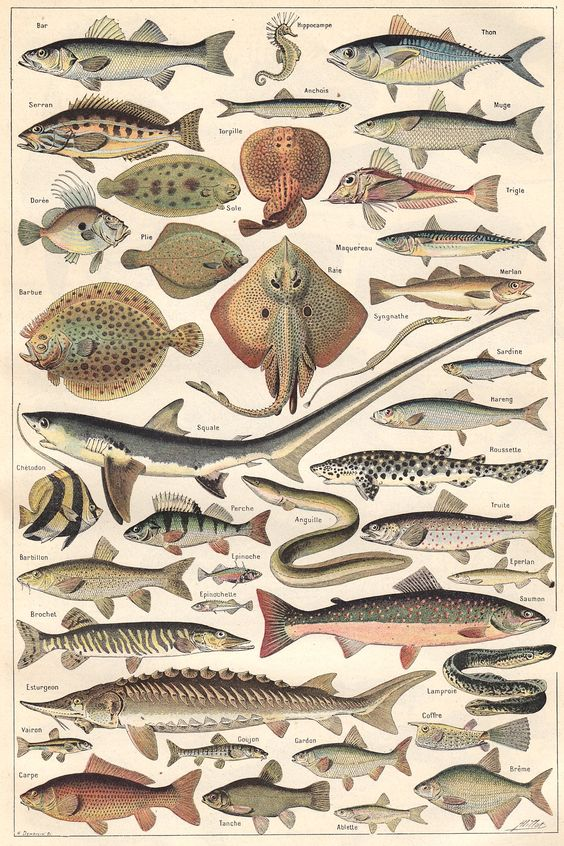
\includegraphics[scale=.25]{figs/species4.jpg}
        \end{column}

        %You can add more columns, but beware, they're get harder to read the more you add.
    \end{columns}
\end{frame}

%%%%%%%%%%%%%%%%%%%%%%%%%%%%%%%%%%%%%%%%%%%%%%

% FRAME 
\begin{frame}{Theorems and Proofs}
    Theorems and proofs appear differently in a Beamer presentation than they do normally.
    \begin{itemize}
        \item Every aspect of their appearance is customizable and the default depends on your theme.
    \end{itemize}
    
    \begin{theorem}[Soundness of Roundness]
        Every circle has no corners.
    \end{theorem}

    \begin{proof}
        Well, duh.
    \end{proof}
\end{frame}

%%%%%%%%%%%%%%%%%%%%%%%%%%%%%%%%%%%%%%%%%%%%%%

% FRAME 
\begin{frame}
    If you need extra space, you can leave off the title of the slide and the header will not appear.
    This is helpful if you need to create big images or complicated diagrams like this one:

    \begin{center}
        %tikz is a package for creating precise vector graphics in LaTeX. They are created with code--a lot of code. As such, they take up way too much space in your document. A good practice is to put the code for a tikz diagram in its own file and then use the \input function to insert it into your file like this.
        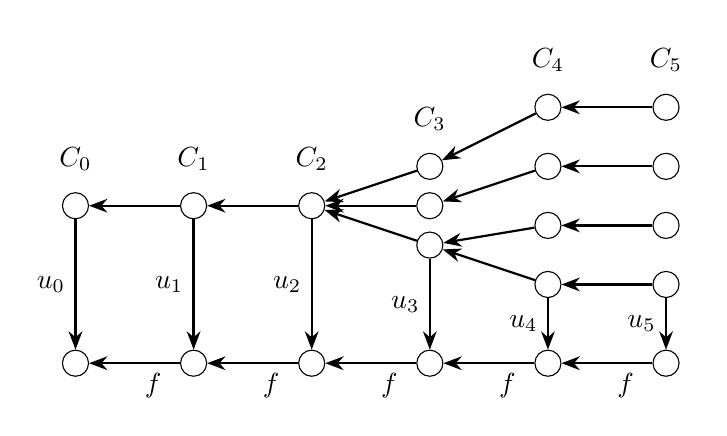
\begin{tikzpicture}
    %There's a lot to learn about how tikz works. I recommend tinkering with this example to get a feel for how it works.
    \begin{scope}[every node/.style={circle,draw}]
        \node [label={$C_0$}](0) at (0,0) {};
        \node [label={$C_1$}](1) at (1.5,0) {};
        \node [label={$C_2$}](2) at (3,0) {};
        \node [label={$C_3$}](31) at (4.5,.5) {};
        \node (30) at (4.5,0) {};
        \node (32) at (4.5,-.5) {};
        \node [label={$C_4$}](41) at (6,1.25) {};
        \node (40) at (6,.5) {};
        \node (42) at (6,-.25) {};
        \node (43) at (6,-1) {};
        \node [label={$C_5$}] (51) at (7.5,1.25) {};
        \node (52) at (7.5,.5) {};
        \node (53) at (7.5,-.25) {};
        \node (54) at (7.5,-1) {};
        
        \node (b0) at (0,-2){};
        \node (b1) at (1.5,-2){};
        \node (b2) at (3,-2){};
        \node (b3) at (4.5,-2){};
        \node (b4) at (6,-2){};
        \node (b5) at (7.5,-2){};
    \end{scope}
    
    \begin{scope} [>={Stealth[black]},
                every node/.style={below right},
                every edge/.style={draw=black, thick}]
        \path [->] (1) edge (0);
        \path [->] (2) edge (1);
        \path [->] (31) edge (2);
        \path [->] (30) edge (2);
        \path [->] (32) edge (2);
        \path [->] (41) edge (31);
        \path [->] (40) edge (30);
        \path [->] (42) edge (32);
        \path [->] (43) edge (32);
        \path [->] (51) edge (41);
        \path [->] (52) edge (40);
        \path [->] (53) edge (42);
        \path [->] (54) edge (43);
        
        \path [->] (b5) edge node {$f$} (b4);
        \path [->] (b4) edge node {$f$} (b3);
        \path [->] (b3) edge node {$f$} (b2);
        \path [->] (b2) edge node {$f$} (b1);
        \path [->] (b1) edge node {$f$} (b0);
    \end{scope}
    
    \begin{scope}[>={Stealth[black]},
                every node/.style={left},
                every edge/.style={draw=black,  thick}]
        \path [->] (0) edge node {$u_0$} (b0);
        \path [->] (1) edge node {$u_1$} (b1);
        \path [->] (2) edge node {$u_2$} (b2);
        \path [->] (32) edge node {$u_3$} (b3);
        \path [->] (43) edge node {$u_4$} (b4);
        \path [->] (54) edge node {$u_5$} (b5);
    \end{scope}
    
\end{tikzpicture}
    \end{center}

\end{frame}

%%%%%%%%%%%%%%%%%%%%%%%%%%%%%%%%%%%%%%%%%%%%%%

% FRAME 
\begin{frame}
Here's another example of the kind of diagram you can make with TikZ.

\begin{center}
    \usetikzlibrary {3d}
\begin{tikzpicture}[z={(10:10mm)},x={(-45:5mm)}]
  \def\wave{
    \draw[fill,thick,fill opacity=.2]
     (0,0) sin (1,1) cos (2,0) sin (3,-1) cos (4,0)
           sin (5,1) cos (6,0) sin (7,-1) cos (8,0)
           sin (9,1) cos (10,0)sin (11,-1)cos (12,0);
    \foreach \shift in {0,4,8}
    {
      \begin{scope}[xshift=\shift cm,thin]
        \draw (.5,0)  -- (0.5,0 |- 45:1cm);
        \draw (1,0)   -- (1,1);
        \draw (1.5,0) -- (1.5,0 |- 45:1cm);
        \draw (2.5,0) -- (2.5,0 |- -45:1cm);
        \draw (3,0)   -- (3,-1);
        \draw (3.5,0) -- (3.5,0 |- -45:1cm);
      \end{scope}
    }
  }
  \begin{scope}[canvas is zy plane at x=0,fill=blue]
    \wave
    \node at (6,-1.5) [transform shape] {magnetic field};
  \end{scope}
  \begin{scope}[canvas is zx plane at y=0,fill=red]
    \draw[help lines] (0,-2) grid (12,2);
    \wave
    \node at (6,1.5) [rotate=180,xscale=-1,transform shape] {electric field};
  \end{scope}
\end{tikzpicture}
\end{center}

\end{frame}

%%%%%%%%%%%%%%%%%%%%%%%%%%%%%%%%%%%%%%%%%%%%%%
% FRAME
\begin{frame}
    \vassarbox{Thanks!}
    \vspace{.2in}
    
    \begin{center}
        For more resources on using Beamer, including templates\\
        
\includegraphics[scale=.1]{figs/beamer_resources.png}
    \end{center}

\end{frame}

\end{document}

%I keep this down here for ease of copy/pasting

%%%%%%%%%%%%%%%%%%%%%%%%%%%%%%%%%%%%%%%%%%%%%%

% FRAME 
\begin{frame}{}

\end{frame}

%%%%%%%%%%%%%%%%%%%%%%%%%%%%%%%%%%%%%%%%%%%%%%